\documentclass[12pt]{report}

%%%%%%%%%%%%%%%%%%%%%%%%%%%%%%%%%%%%%%%%%%%%%%%%%%%%%%%%%%%%%%%%%%%%
% package and document formatting stuff
%%%%%%%%%%%%%%%%%%%%%%%%%%%%%%%%%%%%%%%%%%%%%%%%%%%%%%%%%%%%%%%%%%%%

% symbols and math stuff
\usepackage{amsmath,amsthm,amssymb}
\usepackage{tikz}
\usepackage{tkz-graph}
\usetikzlibrary{arrows,%
                petri,%
                topaths}%

\usepackage{tkz-berge}


% math operators
\usepackage{amsopn}

% script and caligraphics
\usepackage{eucal,mathrsfs}

% indexing
\usepackage{makeidx}

\usepackage{enumerate}

% formatting
\usepackage{fullpage}

% links and colors
\usepackage{color}
\usepackage[pdfstartview=FitH,
%             pdfauthor={\myauthor},
%             pdftitle={\mytitle},
            colorlinks,
            linkcolor=reference,
            citecolor=citation,
            urlcolor=e-mail,
            backref]{hyperref}
\usepackage[all]{xy}

\definecolor{todo}{rgb}{.80,.20,.20}
\definecolor{e-mail}{rgb}{0,.40,.80}
\definecolor{reference}{rgb}{.10,.40,.42}
\definecolor{mrnumber}{rgb}{.80,.40,0}
\definecolor{citation}{rgb}{0,.40,.80}

%%%%%%%%%%%%%%%%%%%%%%%%%%%%%%%%%%%%%%%%%%%%%%%%%%%%%%%%%%%%%%%%%%%%
% theorem stuff
%%%%%%%%%%%%%%%%%%%%%%%%%%%%%%%%%%%%%%%%%%%%%%%%%%%%%%%%%%%%%%%%%%%%

\theoremstyle{plain}

\newtheorem{thm}{Theorem}[section]
\newtheorem{defn}[thm]{Definition}
\newtheorem{deflem}[thm]{Definition/Lemma}
\newtheorem{notn}[thm]{Notation}
\newtheorem{convention}[thm]{Convention}
\newtheorem{lem}[thm]{Lemma}
\newtheorem{aside}[thm]{Aside}
\newtheorem{rem}[thm]{Remark}
\newtheorem{ex}[thm]{Example}
\newtheorem{facts}[thm]{Facts}
\newtheorem{cor}[thm]{Corollary}
\newtheorem{conj}[thm]{Conjecture}
\newtheorem{prop}[thm]{Proposition}

\newtheorem{question}[thm]{Question}
\newtheorem{exercise}{Exercise}[section]

%%%%%%%%%%%%%%%%%%%%%%%%%%%%%%%%%%%%%%%%%%%%%%%%%%%%%%%%%%%%%%%%%%%%
% typography stuff
%%%%%%%%%%%%%%%%%%%%%%%%%%%%%%%%%%%%%%%%%%%%%%%%%%%%%%%%%%%%%%%%%%%%

\newcommand{\mb}[1]{\mathbf #1}
\newcommand{\mbb}[1]{\mathbb #1}
\newcommand{\mf}[1]{\mathfrak #1}
\newcommand{\mc}[1]{\mathcal #1}
\newcommand{\ms}[1]{\mathscr #1}
\newcommand{\mcu}[1]{\mathcu #1}
\newcommand{\oper}[1]{\operatorname{#1}}

\newcommand{\da}{\downarrow}
\newcommand{\ra}{\rightarrow}
\newcommand{\hra}{\hookrightarrow}
\newcommand{\dra}{\dashrightarrow}
\newcommand{\la}{\leftarrow}
\newcommand{\lra}{\longrightarrow}

\newcommand{\ov}{\overline}
\newcommand{\til}{\widetilde}
\newcommand{\wh}{\widehat}

\newcommand{\ZZ}{\mathbb{Z}}

\newcommand{\ann}{\oper{ann}}
\newcommand{\coker}{\oper{coker}}
\newcommand{\End}{\oper{End}}
\newcommand{\Aut}{\oper{Aut}}
\newcommand{\Stab}{\oper{Stab}}

\newcommand{\ind}{\oper{ind}}
\newcommand{\per}{\oper{per}}
\newcommand{\cores}{\oper{cor}}

\newcommand{\Br}{\oper{Br}}
\newcommand{\quat}[3]{
  \left(\begin{matrix} #1, #2 \\ #3
  \end{matrix}\right)
}
\newcommand{\symb}[3]{
  \left(#1, #2\right)_{#3}
}

\newcommand{\lcm}{\oper{lcm}}

%%%%%%%%%%%%%%%%%%%%%%%%%%%%%%%%%%%%%%%%%%%%%%%%%%%%%%%%%%%%%%%%%%%%
% other stuff
%%%%%%%%%%%%%%%%%%%%%%%%%%%%%%%%%%%%%%%%%%%%%%%%%%%%%%%%%%%%%%%%%%%%

\makeindex
\newcommand{\X}[1]{#1\index{#1}}
\newcommand{\Xb}[1]{\textbf{#1}\index{#1}}
\newcommand{\Ab}[2]{\textbf{#1}\index{#2}}

\newcommand{\todo}[1]{\textcolor{todo}{#1}}

%%%%%%%%%%%%%%%%%%%%%%%%%%%%%%%%%%%%%%%%%%%%%%%%%%%%%%%%%%%%%%%%%%%%
% end preamble
%%%%%%%%%%%%%%%%%%%%%%%%%%%%%%%%%%%%%%%%%%%%%%%%%%%%%%%%%%%%%%%%%%%%

\begin{document}

%%%%%%%%%%%%%%%%%%%%%%%%%%%%%%%%%%%%%%%%%%%%%%%%%%%%%%%%%%%%%%%%%%%%
% title stuff
%%%%%%%%%%%%%%%%%%%%%%%%%%%%%%%%%%%%%%%%%%%%%%%%%%%%%%%%%%%%%%%%%%%%


\author{Daniel Krashen}
\title{Graph Theory}

\maketitle
\tableofcontents

%%%%%%%%%%%%%%%%%%%%%%%%%%%%%%%%%%%%%%%%%%%%%%%%%%%%%%%%%%%%%%%%%%%%
% document stuff
%%%%%%%%%%%%%%%%%%%%%%%%%%%%%%%%%%%%%%%%%%%%%%%%%%%%%%%%%%%%%%%%%%%%

\chapter*{Version Notes}
\addcontentsline{toc}{chapter}{Version Notes}

\section{Updates 1/28/2016}
\begin{itemize}
\item added Section~\ref{other basic notions section}, to introduce some
additional notation
\item added spanning subgraph material (some) in Section~\ref{lecture 5}
\end{itemize}

\section{Updates 1/30/2016}
\begin{itemize}
\item added Lemma~\ref{dijkstra optimality}
on the optimality of Dijkstra's algorithm.
\item reorganized exercises (to ends of chapters)
\end{itemize}

\section{Updates 2/07/2016}
\begin{itemize}
\item add Chapter~\ref{chap:more connectivity}
\item defined trivial graphs: Definition~\ref{def:trivial}
\item added definition of underlying simple graph:
Definition~\ref{def:underlying simple graph}
\end{itemize}


\chapter{Lecture 1: The language of graphs}

\section{Graphs}
Graphs encode the idea of connections between things, for example
\begin{itemize}
\item networks of computers
\item people and their relationships
\item cities and highways
\item sets and intersections
\item workers and tasks
\end{itemize}


In formal mathematical terms, a graph is:
\begin{defn}
A \Xb{graph} $G$ is an ordered triple $(V, E, \psi)$ consisting of
\begin{itemize}
\item a finite, nonempty set $V$, whose elements are referred to as vertices,
\item a finite (possibly empty) set $E$, whose elements are referred to as
edges, and
\item an ``incidence'' function $\psi: E \to \ms R_2(V)$,
\end{itemize}
where $\ms R_2(V)$ is the set of unordered pairs of elements of $V$ (which
one may also think of as two elements multisubsets of $V$ -- see
Definition~\ref{multisubsets definition}).
\end{defn}

We represent such graphs visually by drawing vertices as dots or circles,
and edges as lines between them. For example, the drawing in
Figure~\ref{basic graph} would stand for the graph $G$ defined by $V_G =
\{A, B, C, D\}, E_G = \{1, 2, 3, 4, 5\}$ and incidence function $\psi_G$
given by:
\[\psi_G(1) = AC, \ \psi_G(2) = BC, \ \psi_G(3) = CD, \ \psi_G(4) = AD, \
\psi_G(5) = BD.\]

\begin{figure} \label{basic graph}
\caption{}
\begin{center}
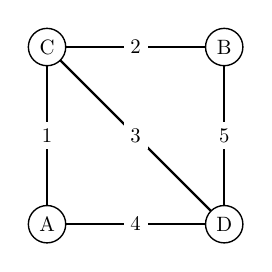
\begin{tikzpicture}[scale=0.75,transform shape]
  \Vertex[x=0,y=0]{A}
  \Vertex[x=3,y=3]{B}
  \Vertex[x=0,y=3]{C}
  \Vertex[x=3,y=0]{D}

  \tikzstyle{LabelStyle}=[fill=white]

  \Edge[label=$1$](A)(C)
  \Edge[label=$2$](B)(C)
  \Edge[label=$3$](C)(D)
  \Edge[label=$4$](D)(A)
  \Edge[label=$5$](B)(D)
\end{tikzpicture}
\end{center}
\end{figure}

\begin{notn}
For a graph $G = (V, E, \psi)$ we write $V_G$ for $V$, $E_G$ for $E$ and
$\psi_G$ for $\psi$.
\end{notn}
In other words, using this notational convention, if we are given graphs
$G, H, K$, and have not specified letters for their sets of vertices,
edges, etcetera, we may write, for example, $E_K$ for the edges of the
graph $K$, $V_H$ for the vertices of $H$, and $\psi_G$ for the incidence
function of $G$.

\begin{defn} \label{def:trivial}
A graph is called \textbf{trivial}\index{graph!trivial} if it has a single
vertex (see Figure~\ref{fig:some trivial graphs}).
\end{defn}

\begin{defn}
Let $G$ be a graph, $e \in E_G$ an edge and $v \in V_G$ a vertex. We say
that $e$ and $v$ are \Xb{incident} if $v \in \psi(e)$.
\end{defn}

\begin{defn}
Let $G$ be a graph $v, w \in V_G$. We say that $v$ and $w$ are
\Xb{adjacent} if there is an edge $e$ with $v$ and $w$ incident to
$e$.
\end{defn}

\begin{defn}
Let $G$ be a graph $e, e' \in E_G$. We say that $e$ and $e'$ are
\Xb{adjacent} if there is a vertex $v$ with $e$ and $e'$ incident to
$v$.
\end{defn}

DIAGRAM

\begin{defn}
Let $G$ be a graph. If $e \in E_G$ is an edge, we say that $e$ is a
\Xb{loop}, if $e$ is incident to exactly one vertex.
\end{defn}

\begin{defn}
Let $G$ be a graph. If $e \in E_G$ is an edge, we say that $e$ is an
\Xb{arc}, if $e$ is incident to exactly two vertices.
\end{defn}

\begin{defn}
We say that $G$ is a \Xb{simple graph} if
\begin{itemize}
\item $G$ has no loops,
\item there is at most $1$ edge incident to any pair of vertices.
\end{itemize}
\end{defn}
Note that the second condition is the same as requiring that the function
$\psi_G$ be one-to-one.

Graphs can be drawn in many different ways:

\begin{defn}
$G$ is called a \Xb{planar graph} if it may be drawn in the plane with no
edges crossing.
\end{defn}



\section{Real world graph problems}

In the section we'll consider some classic problems which translate
naturally to graph theory.

\subsection{Scheduling}
\begin{itemize}
\item vertices = jobs that need to be done
\item edges = jobs which require conflicting resources
\end{itemize}
problem: how to decide how many ``periods of work'' needed to complete
all jobs.

Similar problem: table arrangements at a wedding
\begin{itemize}
\item vertices = guests
\item edges = guest that don't get along
\end{itemize}
problem: how many tables?

translation: vertex colorings, chromatic number of a graph
\begin{defn}
A \Xb{vertex coloring} of a graph $G$ is a function $f$ defined on the set of
vertices of $G$. An vertex $n$-coloring is a function $f : V_G \to \{1,
\ldots, n\}$. We say that a vertex coloring is \textbf{proper}\index{vertex
coloring!proper} if $f(v) \neq f(w)$ for adjacent vertices $v, w$.
\end{defn}

\begin{defn}
The chromatic number of a graph, $\chi(G)$, is the minimal number $n$ such
that $G$ has a proper vertex $n$-coloring.
\end{defn}

\subsection{Tournaments}

various teams need to play each other. disjoint pairs of teams can play
simultaneously, but of course the same team can't play at the same time.
How many rounds are needed for teams to play each other?
\begin{itemize}
\item vertices = teams
\item edges = teams who need to play each other
\end{itemize}
problem: how many rounds?

\begin{defn}
An \Xb{edge coloring} of a graph $G$ is a function $f$ defined on the set of
edges of $G$. An edge $n$-coloring is a function $f : E_G \to \{1,
\ldots, n\}$. We say that an edge coloring is \textbf{proper}\index{proper!edge
coloring} if $f(e) \neq f(e')$ for adjacent vertices $e, e'$.
\end{defn}

\begin{defn}
The \Xb{edge chromatic number} of a graph, $\chi'(G)$, is the minimal
number $n$ such that $G$ has a proper edge $n$-coloring.
\end{defn}


\section{The rationale behind the language}

The choice of thinking of a graph as a triple $G = (V, E, \psi)$ has its
advantages and disadvantages. If we were only concerned with simple graphs,
we could have simplified our notation somewhat by omitting the function
$\psi$, and letting $E$ itself be a subset of the set of 
unordered pairs of distinct elements of $V$. In the case of general graphs,
however, where there can be multiple edges between two vertices, this is
somewhat less convenient. We could persist with this approach by saying
that $E$ be a multisubset instead of a subset, however, this is a little
bit less convenient later when we wish to talk about colorings or
labellings of edges.

An alternate way of defining things could be as follows: Instead of
defining the function $\psi$ as the fundamental concept, one may instead
define the notion of \textbf{incidence} as the fundamental concept as
follows:

\begin{defn} \label{griph}
A griph $G$ is an ordered triple $(V, E, \alpha)$ consisting of a set of
vertices $V$, a set of edges $E$, and a set of ordered pairs $\alpha
\subset V \times E$ such that \item for every $e \in E$, there is at least
one, and at most two elements $v \in V$ such that $(v, e) \in \alpha$. If
$(v, e) \in \alpha$, we say that $v$ is incident to $e$. A griph is called
simple if every edge is incident to exactly two vertices.
\end{defn}



\section{Other basic notions} \label{other basic notions section}

For a graph $G$, we let $v(G) = \#V_G$ denote the number of vertices of
$G$, and $e(G) = \#E_G$ denote the number of edges of $G$. We let
$\delta(G)$ denote the mininum degree of a vertex of $G$, and $\Delta(G)$
denote the maximum degree of a vertex.


\section{Exercises}

\begin{exercise}
Show that griphs are exactly in correspondence with graphs in such a way
that the relationship of incidence lines up.
\end{exercise}


\chapter{Lecture 2: Digraphs and degree formulas}
\section{Directed graphs}

A variation on the notion of a graph is also very useful both theoretically
and in applications:

\begin{defn}
A \Xb{directed graph} or \Ab{digraph}{digraph|see {directed graph}} $D$ is an
ordered triple $(V, A, \psi)$ where $V$ is a set, referred to as the
\textbf{vertices} of $D$, a set $A$ referred to as the \Xb{arrows} of $D$,
and a pair of functions $s, t: A \to V$, taking arrows to
elements of $V$.
\end{defn}

\begin{notn}
For a digraph $D = (V, A, \psi)$, as before, we write $V_D$ for $V$, $A_D$
for $A$, $s_D$ for $s$, and $t_D$ for $t$.
\end{notn}

\begin{notn}
For a digraph $D$, and an arrow $a \in A_D$, we call $s(a)$ the
\Ab{source}{source (of an arrow)} of $a$ and $t(a)$ the \Ab{target}{target
(of an arrow)} of $a$.
\end{notn}

EXAMPLES:
\begin{itemize}
\item one way street maps
\item irreversible processes
\item dependencies: e.g. scheduling with dependencies
\end{itemize}

\newcommand{\outdeg}{\oper{outdeg}}
\newcommand{\indeg}{\oper{indeg}}

\begin{defn} \label{inoutdegree}
Let $D$ be a digraph. For a vertex $v$, we define the \Xb{outdegree} of
$v$, denoted $\outdeg v$, to be the number of edges whose source is $v$,
and the \Xb{indegree} of $v$, denoted $\indeg v$, to be the number of edges
whose target is $v$.
Formall, we have
\[ \outdeg v = \#\{a \in A_D \mid  s(a) = v\} ,\ \ 
\indeg v = \#\{a \in A_D \mid t(a) = v\}.
\]
If it is necessary to specify the digraph, we may also write $\outdeg_D(v)$
or $\indeg_D(v)$.
\end{defn}

\begin{prop}[The degree formula for digraphs]
Suppose that $D$ is a digraph. Then 
\[\sum_{v \in V_D} \outdeg(v) = \sum_{v \in V_D} \indeg(v) = \#A_D.\]
\end{prop}
\begin{proof}
Informally, this is clear for the following reason: every arrow in $A_D$
has its source at exactly one vertex, and so contributes exactly $1$ to the
first sum, and every arrow has its target at exactly one vertex and
similarly contributes exactly once to the second sum.

Let us, however, for the sake of practice, give a more formal argument:
\[\sum_{v \in V_D} \outdeg(v) = \sum_{v \in V_D} \sum_{a \in A_D, s(a) = v}
1 = \sum_{(v, a) \in V_D \times A_D, s(a) = v} 1 \]
But now, let us notice that the pairs $(v, a)$ with $s(a) = v$ are in
bijection with simply the set $A_D$, since by the description, $v$ is
determined by $a$. Therefore, we may rewrite this as:
\[\sum_{(v, a) \in V_D \times A_D, s(a) = v} 1  = \sum_{a \in A_D} 1 =
\#A_D.\]
The rest of the proof follows in an analogous way.

\end{proof}

\section{From graphs to digraphs}

Given a graph $G$, we may construct a digraph $dig(G)$ by definining
\begin{itemize}
\item $V_{dig(G)} = V_G$,
\item $A_{dig(G)} = \{(v, e) \in V \times E | v \in \psi(e)\}$,
\item $s_{dig(G)}(v, e) = v$, $t_{dig(G)}(v, e) = w$, where $\psi(e) = vw$.
\end{itemize}

\begin{defn}
Suppose that $G$ is a graph. We define the \Xb{degree} of a vertex $v \in
V_G$, denoted $\deg v$ to be the number of edges incident to $v$. If it is
necessary to specify the graph, we may also write $\deg_G v$.
\end{defn}

\begin{prop}[The degree formula for graphs]\label{degree formula}
Suppose that $G$ is any graph. Then we have
\[\sum_{v \in V_G} \deg v = 2\#E.\]
\end{prop}
\begin{proof}
Intuitively, one way to see this is that if we chop each edge in the
middle, making two ``half edges'' for every edge, then each half edge is
incident to exactly one vertex, and contritutes exactly once to the degree
count on the left.

More formally, if we let $dig(G)$ be the associated digraph to $G$, then we
note that for every edge of $G$, there are two arrows of $dig(G)$. Also,
for every edge $e$ incident to $v$, there is exactly one arrow, which we
call $(v, e)$ which starts at $e$. That is, the map
\begin{align*}
\{e \in E_G | \text{$e$ is incident to $v$}\} &\to \{a \in A_{dig(G)} | s(a)
= v\} \\
e \mapsto (v, e) 
\end{align*}
is a bijection (its inverse being given by $(v, e) \mapsto e$). In
particular, this says that $\outdeg_{dig(G)} v = \deg_G v$.

By the
degree formula for digraphs, we therefore have
\[\sum_{v \in V_G} \deg_G v = \sum_{v \in A_{dig(G)}} \outdeg_{dig(G)} v =
\#A_{dig(G)} = 2\#E_G\]
as desired.
\end{proof}

A surprising conclusion here is that the sum of the degrees of the vertices
of a graph must be even! 

\section{Exercises}

\chapter{Lecture 3: Subgraphs, isomorphisms}

\section{Isomorphisms}

\begin{defn}
Given two graphs $G, H$, an \Xb{isomorphism} $f$ from $G$ to $H$, written
$f: G \to H$ is a pair of maps $f = (f_V, f_E)$, where $f_V: V_G \to V_H$
is a function from the vertices of $G$ to the vertices of $H$ and $f_E: E_G
\to E_H$ is a function from the edges of $G$ to the edges of $H$ such that
both $f_V$ and $f_E$ are bijective and such that for $v \in V_G$, $e \in
E_G$, we have that $v$ and $e$ are incident if and only if $f_V(v)$ is
incident to $f_E(e)$.
\end{defn}

\begin{notn}
If $G$ and $H$ are graphs, we write $G \cong H$ and say that $G$ and $H$
are \textbf{isomorphic}\index{isomorphic graphs} if there exists an
isomorphism $f: G \to H$.
\end{notn}

In other words, thinking of the sets $V_G, E_G$ as the labels for the
vertices and edges of $G$ and thinking of $V_H, E_H$ as the labels for the
vertices and edges of $H$, we may think of $f_V$ and $f_E$ as re-assigning
the labels of the vertices and edges of a graph. The final property says
that the relation of incidence is preserved. Note that the incidence
relation encodes the function $\psi$, as $v$ and $e$ are incident if and
only if $v \in \psi(e)$ (and since the unordered pair/two element multiset
$\psi(e)$ is determined precisely by which elements it contains).

This is very useful, as our main concern is structural information about
graphs, as opposed to the specific names which we have assigned to their
edges and vertices. For this reason, when drawing a graph, we will
typically omit names for the vertices and edges, drawing our graphs as in
figure~\ref{fig:graph examples} instead.

\begin{figure} \label{fig:graph examples}
\begin{center}
\caption{some graphs}

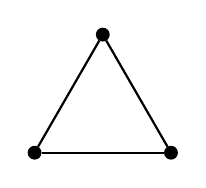
\begin{tikzpicture}[rotate=90] 
  \tikzset{VertexStyle/.style = {shape = circle,fill = black,minimum size =
  5pt,inner sep=0pt}}
  \Vertices[NoLabel]{circle}{A,B,C}
  \Edges(A,B,C,A)
\end{tikzpicture}
\hspace{1cm}
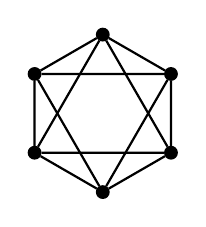
\begin{tikzpicture}[rotate=30] 
  \tikzset{VertexStyle/.style = {shape = circle,fill = black,minimum size =
  5pt,inner sep=0pt}}
  \Vertices[NoLabel]{circle}{a, b, c, d, e, f}
  \Edges(a, b, c, d, e, f, a)
  \Edges(a, c, e, a)
  \Edges(b, d, f, b)
\end{tikzpicture}
\hspace{1cm}
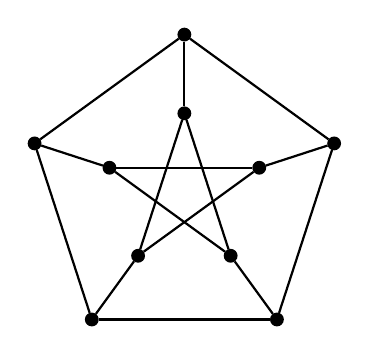
\begin{tikzpicture}[rotate=90]
  \GraphInit[vstyle=simple]
  \tikzset{VertexStyle/.style = {shape = circle,fill = black,minimum size =
  5pt,inner sep=0pt}}
  \grPetersen[RA=2,RB=1]
\end{tikzpicture}
\end{center}
\end{figure}

\subsection{Simplifications for simple graphs}
It is perhaps useful to note that this definition may be made a bit simpler
in the case of simple graphs (not suprising, I'm sure). To be precise:

Expanding on this idea a bit, we see that in a simple graph, the graph is
determined up to isomorphism by the relationship of adjacency -- that is,
which vertices are joined by an edge. That is to say, although these two
graphs shown in Figure~\ref{fig:isomorphism example} are different as
graphs, they are still isomorphic canonical way, via the labelling of the
vertices. 

\begin{figure} \label{fig:isomorphism example}
\caption{isomorphic graphs}
\begin{center}
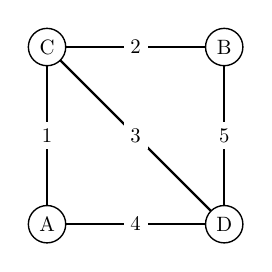
\begin{tikzpicture}[scale=0.75,transform shape]
  \Vertex[x=0,y=0]{A}
  \Vertex[x=3,y=3]{B}
  \Vertex[x=0,y=3]{C}
  \Vertex[x=3,y=0]{D}

  \tikzstyle{LabelStyle}=[fill=white]

  \Edge[label=$1$](A)(C)
  \Edge[label=$2$](B)(C)
  \Edge[label=$3$](C)(D)
  \Edge[label=$4$](D)(A)
  \Edge[label=$5$](B)(D)
\end{tikzpicture}
\ \ \ \ 
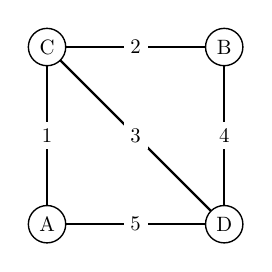
\begin{tikzpicture}[scale=0.75,transform shape]
  \Vertex[x=0,y=0]{A}
  \Vertex[x=3,y=3]{B}
  \Vertex[x=0,y=3]{C}
  \Vertex[x=3,y=0]{D}

  \tikzstyle{LabelStyle}=[fill=white]

  \Edge[label=$1$](A)(C)
  \Edge[label=$2$](B)(C)
  \Edge[label=$3$](C)(D)
  \Edge[label=$5$](D)(A)
  \Edge[label=$4$](B)(D)
\end{tikzpicture}
\end{center}
\end{figure}



\begin{notn}
Along the same lines, for a
simple graph $G = (V, E, \psi)$, if $e$ is an edge with $\psi(e) = vw$, we
will abuse language and refer to $vw$ as $e$. In other words, the statement
that for a pair of vertices $v, w \in V$, $vw \in E$ means that there is
some edge $e$ with $\psi(e) = vw$, or equivalently $v$ and $w$ are
adjacent.
\end{notn}


\begin{defn}
For a simple graph $G$, we define the \textbf{complement}\index{complement
of a simple graph} $G$, denoted $\ov G$ to be the graph with the same set
of vertices (i.e. $V_G = V_{\ov G}$) and such that a pair of vertices $v,
w$ are adjacent in $\ov G$ if and only if they are \textit{not} adjacent in
$G$.
\end{defn}

Associated to an arbitrary graph $G$, one may associate a simple graph
$|G|$,
called the \Xb{underlying simple graph} of $G$. This new graph has the same
vertex set as $G$, and is obtained
by deleting all loops of the original graph and by having a single edge $e$
between vertices whenever they are adjacent in $G$. More precisely, we have 
\begin{defn} \label{def:underlying simple graph}
Let $G$ be a graph. We define the graph $|G|$ via:
$V_{|G|} = V_G$, and 
\[E_{|G|} = \{ uv \in \ms R_2(G) \mid \text{ $u$ is adjacent to $v$ in $G$
}\}\] with $\psi_{|G|}(uv) = uv$.
\end{defn}

\section{Subgraphs}

\begin{defn}
Let $G$ be a graph. We say that a graph $H$ is a \Xb{subgraph} of a graph
$G$ if $V_H \subset V_G$, $E_H \subset E_G$ and $\psi_H = \psi_G|_{E_H}$.
If $H$ is a subgraph of $G$, we write $H \subset G$.
\end{defn}

\begin{defn}
Let $G$ be a graph, and $W \subset V_G$ a subset of its vertices. We
define a new graph $G[W]$, called \textbf{the subgraph of $G$ induced by
$W$}\index{induced subgraph}, to be the graph whose vertex set is $W$ and
whose edge set $E_{G[W]}$ consists of all the edges of $G$ which are only
incident to vertices in $W$, together with the same incidence relations.
Formally, we set
\[ V_{G[W]} = W, \ E_{G[W]} = \{ e \in E_G \mid \psi(e) \subset W\}, \
\psi_{G[W]} = \psi|_{E_{G[W]}},\]
where $\psi|_{E_{G[W]}}$ denotes the restriction of the function $\psi$ to
the edges of $G[W]$.
\end{defn}

Given a graph $G$, we will often want to understand its structure by
looking at which subgraphs it has, and their properties. For example,
consider the following famous statement:

\begin{quote}
In every group of $6$ people, there is either a group of $3$ people all of
whom know each other, or a group of $3$ people, none of whom know each
other.
\end{quote}

One convenient way of conceptualizing this question within the framework of
graph theory is as follows: consider the two special graphs below

TRIANGLE   \ \ \ \ \ \ DISCRETE GRAPH WITH 3 VERTICES

We may now formally state the previous result as follows:

In generalizing this result, which we will look into later in
Chapter~\ref{ramsey chapter}, it is natural to want to consider groups of
$n$ vertices in a graph, all of which are connected. The correponding
subgraphs of interest are called the complete graphs:

\begin{defn}
The \Xb{complete graph} on $n$ vertices, denoted $K_n$ is the simple graph
with vertices consisting of the set $\{1, \ldots, n\}$, and where every two
vertices are adjacent.
\end{defn}

\begin{defn}
Let $G$ be a simple graph. An $n$-\Xb{clique} in $G$ is a collection of
vertices $v_1, \ldots, v_n \in V_G$ such that the induced subgraph
$G[\{v_1, \ldots, v_n\}]$ is isomorphic to $K_n$.
\end{defn}

It is very natural to ask, for a given graph, about the existence or
non-existence of cliques of a given size -- see, for example exercise
\label{ramsey 6}.

Another way to generalize the graph $K_3$ is in the notion of a cycle graph:
\begin{defn}
The \Xb{cycle graph} on $n$ vertices ($n \geq 3$)\footnote{we let bigons be
bigons, as they say}, denoted $C_n$ is the simple graph with vertices
consisting of the set $\{1, \ldots, n\}$, and where vertices $i$ and $j$
are adjacent if and only if $|i - j|$ is $1$ or $n-1$.
\end{defn}
In other words, there are edges between vertices which are $1$ unit apart,
and one additional edge connecting $1$ and $n$.

\begin{defn}
A cycle in a (not necessarily simple) graph $G$ is a subgraph $C \subset G$
such that $C \cong C_n$ for some $n \geq 3$.
\end{defn}

As we will see, cycles and cliques are interesting for a variety of
reasons, both practically and theoretically. Intuitively,
one should view the existence of cycles and cliques as helping to describe
how highly connected a graph is, somehow encapsulating ``redundancies of
connections.'' We will explore these ideas more in Chapters~\ref{bridges,
circuits, etc}.

\section{Unions, Intersections}

\begin{defn}
Let $G$ be a graph and $H_1, H_2$ sugraphs of $G$. We say that $G$ is the
\textbf{union}\index{union (of graphs)} of $H_1$ and $H_2$, and write $G = H_1
\cup H_2$ if $V_G = V_{H_1} \cup V_{H_2}$ and $E_G = E_{H_1} \cup
E_{H_2}$. We say that the union is \textbf{disjoint}\index{union!disjoint}
if $V_{H_1} \cap V_{H_2} = \emptyset$, and we say that the union is
\textbf{edge disjoint}\index{union!edge disjoint} if $E_{H_1} \cap
E_{H_2} = \emptyset$.
\end{defn}
Note that a disjoint union is automatically edge disjoint as well, since if
two subgraphs share a common edge it must also share any vertices which are
incident to it. Note also that whenever we have any two subgraphs $H_1,
H_2$ in a graph $G$, we may find a unique subgraph $H < G$ with $H = H_1
\cup H_2$. 

\begin{defn} \label{intersection definition}
Let $G$ be a graph and $H_1, H_2 < G$ subgraphs of $G$. We define the
\textbf{intersection}\index{intersection (of graphs)} $H_1 \cap
H_2$ to be the subgraph with $V_{H_1 \cap H_2} = V_{H_1} \cap V_{H_2}$ and
$E_{H_1 \cap H_2} = E_{H_1} \cap E_{H_2}$. 
\end{defn}

\section{Other operations on graphs}

\subsection{adding and removing edges and vertices}

\begin{defn}
Let $G$ be a graph, and $e \in E_G$. We define a subgraph $G - e$ of $G$ by
$V_{G - e} = V_G$ and $E_{G - e} = E_G \setminus \{e\}$.
\end{defn}

\begin{defn}
Let $G$ be a graph, and $e \in E_G$. If $H < G$ is a subgraph, we define
the new subgraph $H + e$ to be the subgraph with
\[V_{H + e} = V_H \cup \{v \in G | \text{ $v$ incident to $e$}\}\]
and
\[E_{H + e} = E_H \cup \{e\}\]
\end{defn}

\begin{defn}
Let $G$ be a graph, and $v \in V_G$. We define the subgraph $G - v$ of $G$
to be the induced subgraph $G - v = G[V \setminus \{v \}$. That is, it is
the graph obtained by removing the vertex $v$ as well as all edges incident
to $v$.
\end{defn}

\section{Exercises}

\begin{exercise}
Suppose that $G$ and $H$ are simple graphs. Suppose we have a bijective
function $g: V_G \to V_H$. Then there exists a unique graph isomorphism $f
= (f_V, f_E) : G \to E$ with $f_V = g$ if and only if for every two
vertices $v, w \in V_G$, we have that $v$ is adjacent to $w$ if and only if
$g(v)$ is adjacent to $g(w)$.
\end{exercise}

\begin{exercise}
Show that every simple graph with $6$ vertices must contain an induced
subgraph isomorphic to one of the above graphs\footnote{hint: as a first
step, considering
the friends of one particular person $A$, partitions the other $5$ people into
two groups (friends of $A$ and not friends of $A$), it follows that one of
these two groups must have at least $3$ people}.
\end{exercise}

\begin{exercise} \label{ramsey 6}
Find the smallest number $n$ such that every simple graph with $n$ edges
and $6$ vertices has a $3$-clique.
\end{exercise}

\begin{exercise}
Give an example of a simple graph with 4 vertices and exactly $3$ cycles, and a
graph with $3$ vertices and exactly $2$ cycles.
\end{exercise}

\begin{exercise}
Verify that definition \ref{intersection definition} does in fact give a
well-defined subgraph.
\end{exercise}



\chapter{Lecture 4: Paths, walks, trails, circuits, cycles}

\section{Walks and connectedness}

This chapter will introduce a fair amount of language which will be useful
in subsequent lectures. 

\begin{defn}
A \Xb{walk} $W$ in a graph $G$ is a sequence of alternating vertices and
edges
\[ W = v_1 e_2 v_2 e_3 v_3 \cdots e_n v_n \]
where $v_1, \ldots, v_n \in V_G$, $e_2, \ldots, e_n \in E_G$, and such that
$e_i$ is incident to the vertices $v_{i-1}$ and $v_i$. The vertex $v_1$ is
called the \textbf{origin}\index{origin (of a walk)} and $v_n$ is called
the \textbf{terminus}\index{terminus (of a walk)}.
\end{defn}

\begin{convention}
We will allow a walk to have only a single vertex. That is, the sequence
consisting only of a single vertex $v$ is a valid walk with origin and
terminus $v$. We will not allow a walk to be empty, however.
\end{convention}

\begin{notn}
It is easy to see that if $G$ is a simple graph, a walk $W = v_1 e_2 \cdots
e_n v_n$ is completely determined by its list of vertices. For this reason,
if $G$ is simple, we will generally write $W = v_1 v_2 \cdots v_n$ for
convenience.
\end{notn}

\begin{defn}
Let $G$ be a graph, $v, w \in V_G$. A $(v, w)$-walk is a walk with origin
$v$ and terminus $w$.
\end{defn}

\begin{defn}
Let $G$ be a graph, $W = v_1 e_2 \cdots e_n v_n$ and $W' = v_1' e_2' \cdots
e_m' v_m'$ walks with $v_n = v_1'$. We define the concatenation $WW'$ of
the two walks to be the $(v_1,v_m')$ walk defined by the sequence
\[v_1 e_2 \cdots e_n v_n e_2' v_2' \cdots e_m' v_m \]
\end{defn}

\begin{defn}
Let $G$ be a graph, and $W = v_1 e_2 \cdots e_n v_n$ a walk. We define the
reverse of $W$, denoted $W^{-1}$ to be the walk $v_n e_n v_{n-1} \cdots e_2
v_1$.
\end{defn}

In Exercise~\ref{walk equivalence}, we defined an equivalence relation on
the set $V_G$ of vertices of $G$, by saying that two vertices $v, w$ are
equivalent if there is a $(v,w)$-walk in $G$.

In this way, we find that the set $V_G$ of vertices of $G$ can be written
as a disjoint union of equivalence classes $V_G = \bigcup_{i = 1}^n V_i$.

\begin{defn}
The induced subgraphs $G[V_i]$ are called the \Xb{components} of $G$. The
number $n$ of components of $G$ is denoted $c(G)$. We say that a graph $G$
is \Xb{connected} if it has a single component.
\end{defn}

Note that a graph is a disjoint union of its components, $G = \bigcup_{i =
1}^{c(G)} G[V_i]$.

\subsection{Bridges}

\begin{defn}
We say that $e \in E_G$ is a bridge if $c(G - e) > c(G)$.
\end{defn}

\begin{lem} \label{lem:components plus 1}
Suppose that $e$ is a bridge. Then $c(G - e) = c(G) + 1$.
\end{lem}
\begin{proof}
Let us begin with the case that $c(G) = 1$.  It is easy to see that if $e$
is a bridge, then it cannot be a loop.  In paticular, it is incident to two
distinct vertices $v_1, v_2$.  It is also clear that $e$ must be the unique
edge connecting its two incident vertices.  Let $G_1$ be the connected
component of $v_1$ in $G - e$ and $G_2$ be the connected component of $G_2$
in $G - e$. We claim that $G - e$ is the disjoint union of $G_1$ and $G_2$,
which would prove that $c(G) = 2$ as desired. 

First, we note that $G_1$ and $G_2$ are disjoint, since they consist of
vertices from distinct equivalence clases. Therefore, we need only to show
that every vertex and edge of $G - e$ is either in $G_1$ or $G_2$. 

Let us begin with the vertices. Let $w \in V_G = V_{G - e}$. By
Lemma~\ref{walk to path}, since $G$ is connected, we can find a $(w,
v_1)$-path in $G$.

If $v_2$ arises in this path, then looking at the first part of the path up
to $v_2$ gives a $(w, v_2)$-path in $G$ which does not involve the vertex
$v_1$. In particular, the edge $e$ cannot arise in this path. Therefore,
this path is actually a $(w, v_2)$-path within the connected component of
$v_2$ in $G - e$. That is, we have shown that $w \in V_2$. 

On the other hand, if $v_2$ doesn't arise in this path, the $(w, v_1)$-path
cannot involve the edge $e$, and in particular, shows that $w$ is in $V_1$.

Finally, we check that the every edge of $G - e$ is either in $G_1$ or
$G_2$. Given such an edge $e' \in E_{G - e}$, suppose $v$ is incident to
$e'$. By the above, $v$ is in $G_1$ or $G_2$. Let us suppose that $v \in
V_{G_1}$. Let $w$ be the other (not necessarily distinct) vertex incident
to $e$. We cannot have $w \in V_{G_2}$ since in this case we would have $w
\sim v$, but by definition, they are in different components. Therefore
both of the incident vertices for $e'$ lie in the same component $G_1$, and
by definition of the induced subgraph, the edge $e'$ is in $G_1$ as well.

To complete the proof, consider the case that $G$ may not be connected. In
this case, write $G = \bigcup_{i = 1}^{c(G)} G_i$ as a disjoint union of its
components (as in Exercise~\ref{components exercise}). Then the edge $e$
lies in some particular component, say $e \in G_1$. We have a disjoint
union:
\[ G - e = (G_1 - e) \cup \bigcup_{i = 2}^{c(G)} G_i, \]
and by the above, either $c(G_1 - e)$ is $1$ or $2$. If it is $1$, then
$G_1 - e$ is connected, and $c(G - e) = c(G)$ by Exercise~\ref{components
exercise}.  If it is $2$, then again by Exercise~\ref{components exercise},
we have $c(G - e) = c(G) + 1$.
\end{proof}

\section{Trails, paths, cycles, circuits}

\begin{defn}
A walk $W = v_1 e_2 v_2 \cdots e_n v_n$ in a graph $G$ is called a
\Xb{trail} if all the edges $e_i$ are distinct. It is called a \Xb{path} if
all the vertices $v_i$ are distinct.
\end{defn}
Note that paths are also nessarily trails.

\begin{lem}
Let $v, w$ be vertices of a graph $G$. Suppose that there is a $(v,w)$-walk
in $G$. Then there is a $(v,w)$-path in $G$.
\end{lem}
\begin{proof}
Suppose that $W = v_1 e_2 v_2 \cdots e_n v_n$ is a walk with $v_1 = v$ and
$v_n = w$. Choose $W$ of minimal length. We claim that $W$ is a path.
Supposing it is not, we would have $v_i = v_j$ for some $i < j$. But in
this case, we may consider the new walk $W' = v_1 e_2 \cdots e_{i-1}
v_{i-1} v_i e_{j+1} v_{j+1} \cdots e_n v_n$. By assumption, this is a
shorter walk, contradicting the minimality of $W$. Therefore $W$ is a path
as claimed.
\end{proof}

\begin{defn}
A walk is called \textbf{closed}\index{walk!closed} is its origin and
terminus coincide. A closed walk $W = v_1 e_2 v_2 \cdots e_n v_n e_{n+1}
v_1$ is called a \Xb{circuit} when $v_1 e_2 v_2 \cdots v_n$ is a trail,
and it is called a \Xb{cycle} when $v_1 e_2 v_2 \cdots v_n$ is a path.
\end{defn}

We remark that in the literature, circuits are also called \Xb{tours}.

\begin{rem} \label{rotate closed walk}
Given a closed walk $C = v_1 e_2 v_2 \cdots e_n v_n e_{n+1} v_1$, one can
obtain other closed walks by traversing the same walk starting at a
different vertex. That is, for every $i$ we can consider the walk $v_i
e_{i+1} v_{i+1} \cdots v_n e_{n+1} v_2 e_2 v_2 \cdots v_{i-1} e_i v_i$. In
this way, we see that we can find closed walks starting and ending at any
vertex along the original walk $C$, and traversing the same set of vertices
and edges, and similarly, we can specify the edge with which the walk must
start.
\end{rem}

Note here that there is some notational ambiguity here, as we have defined
a cycle to both be a subgraph isomorphic to $C_n$, as well as a particular
type of walk. Of course the connection is that if $v_1 e_2 v_2 \cdots
e_{n+1} v_1$ is a cycle, then the vertices $v_1, v_2, \ldots, v_n$
together with the edges $e_2, e_3, \ldots, e_{n+1}$ give a subgraph isomorphic
to $C_n$.

\section{Exercises}

\begin{exercise} \label{walk equivalence}
Define a relation on the vertices of a graph $G$ by saying that $v \sim w$
if and only if there exists a $(v, w)$-walk in $G$. Show that this gives an
equivalence relation.
\end{exercise}

\begin{exercise}
Show that $G$ is connected if and only if we cannot find nonempty subgraphs
$H_1, H_2$ such that $G$ is a disjoint union of $H_1$ and $H_2$.
\end{exercise}

\begin{exercise} \label{components exercise}
Somewhat more generally, show that 
\begin{enumerate}[1. ]
\item $c(G)$ is the maximum number such that
we may write $G$ as a disjoint union $G = \cup_{i = 1}^{c(G)} G_i$.
\item If we have $G = \cup_{i = 1}^n G_i$ a disjoint union, where each
subgraph $G_i$ is connected, then the $G_i$ are the connected components of
$G$ and $n = c(G)$. 
\end{enumerate}
\end{exercise}

\begin{exercise} \label{leaf doesn't change components}
Suppose $G$ is a graph and $v \in V_G$ with $\deg(v) = 1$. Then $c(G) = c(G
- v)$.
\end{exercise}

\section{Spanning subgraphs ans regular graphs}

\begin{defn}
Let $H$ be a subgraph of $G$. We say that $H$ is a \Xb{spanning subgraph}
if $V_H = V_G$.
\end{defn}


\begin{defn}
A graph $G$ is called $k$-\Xb{regular} if every vertex $v \in V_G$ has
degree $k$.
\end{defn}

Let's examine $k$ regular simple graphs for small values of $k$. For example, a
$0$-regular graph is graph with no edges (just isolated vertices).

A connected $1$-regular graph is easily seen to consist just of two
vertices joined by a single edge. It follows that a general $1$-regular
graph, being a disjoint union of its components. It follows that for a
graph $G$, a $1$-regular spanning subgraph $H$ corresponds to what is
called a \Xb{matching}, namely, a way of writing the set of vertices $V_G$
as a disjoint union $V_G = \bigcup P_i$ where each $P_i$ is a pair of
distinct adjacent vertices. 

\begin{lem}
A connected $2$-regular simple graph is isomorphic to a cycle graph $C_n$
for some $n$.
\end{lem}

\chapter{Lecture 5: Trees and spanning trees} \label{lecture 5}

In this lecture we will consider spanning subgraphs, focusing on the case
of trees. These
play a very important role for a variety of reasons.

\section{Trees}

\begin{defn}
We say that a simple graph $G$ is a \Xb{forest}, if it has no cycles; that
is, if it has no subgraphs which are isomorphic to $C_n$, $n \geq 3$.
\end{defn}

\begin{defn}
A \Xb{tree} is a connected forest.
\end{defn}

\begin{defn}
A vertex of degree $1$ in a tree is called a \Xb{leaf}.
\end{defn}


\begin{lem} \label{tree unique path}
A graph $G$ is a tree if and only if there is a unique $(v, w)$-path
between any two vertices.
\end{lem}

\begin{lem} \label{tree count lem}
If $G$ is a tree then $e(G) + 1 = v(G)$.
\end{lem}
We will later see that the converse of this statement is true as well for a
connected graph.
\begin{proof}
Let us first show that this equality holds for all trees. Assuming first
that it doesn't, we may find a tree $T$ with a minimum number of edges such
that the equality doesn't hold. Of course, we can easily see that a
counterexample would have to have at least one edge $e$. Consider the new
graph $T - e$. This graph cannot be connected: if $v, w$ are the vertices
incident to $e$, then in $T$, since $v e w$ is a path from $v$ to $w$, it
is the unique one. But if $T -  e$ were connected, a $(v, w)$-path in $T -
e$ would give a $(v, w)$-path in $T$ which didn't involve $e$,
contradicting uniqueness.

We therefore have by Lemma~\ref{lem:components plus 1} that $T - e$ is a
disjoint union of two connected graphs $T - e = T_1 \cup T_2$. Since $T -
e$ is acyclic, $T_1, T_2$ must be as well, and therefore they are both
trees. By assumption of minimality of $T$, it follows that we have $e(T_1)
+ 1 = v(T_1)$ and $e(T_2) + 1 = v(T_2)$. But therefore we have
\[ e(T) + 1 = \big(e(T_1) + e(T_2) + 1\big) + 1 = e(T_1) + 1 + e(T_2) +
1 = v(T_1) + v(T_2) = v(T) \]
as desired.
\end{proof}

\section{Dijkstra's algorithm}

Consider the following problem. Given a list of cities $c_1, c_2, \ldots,
c_n$ and routes connecting certain cities, find the shortest route between
two given cities $c_i$ and $c_j$.

We can model this problem by letting the cities correspond to vertices of a
connected graph $G$, and by letting the routes be the edges. To keep track of
distances, we add the extra information of some ``cost function:''
\[ w: E_G \to \mathbb R_{\geq 0}\]

We may then ask the following question:
\begin{question}
Given vertices $v, w \in V_G$, how do we find the shortest path between $v$
an $w$.
\end{question}
In practical sitations, particularly when the number of cities and paths is
fairly large, it is not going to be effective to simply start listing paths
in a brute force way. One should also consider how the information of the
graph should be stored and accessed, for example on a computer. For
example, if we represent the graph as a triple, as we have previously
defined, this is not going to be particularly practical from the standpoint
of implementation. For example, suppose we are starting at a vertex $v$ and
would like to start constructing our path. We would first have to start to
look down our list of edges, and for every edge $e$, check and see whether
or not $v$ is incident to $e$, using the incidence function $\psi$. This is
a great deal of work to do for every edge in the graph. Instead, it would
be significantly more 
practical for this type of application to represent the graph as a list
of tuples $L_v = (v, (e_1, v_1), (e_2, v_2), \ldots, (e_n, v_n))$, where the
$e_i$ are the edges incident to $v$, and where $v, v_i$ are the vertices
incident to $e_i$. In this way, starting from a vertex $v$, would mean
starting with the list $L_v$, and being able to immediately access all
incident edges, and look up the corresponding adjacent vertex in order to
continue to build the path.

Let us not describe how to solve this problem. Starting from a vertex $v$,
if we are searching for paths to eventually get to $w$, we will, in the
process, successively build paths in various directions from $v$, finding
minimal length paths to various other vertices in the graph, until we
eventually reach our desired vertex $w$. In particular, the algorithm
really will construct minimal length paths from a fixed starting vertex $v$
to \textit{all} other vertices of the graph. We are free, however, to stop
the process once we have constructed a path to $w$.

How does this all relate to trees? Well, implicit in the process, we will
be constructing \textit{unique} paths from $v$ to every other vertex,
inductively. This will in fact result in building a spanning subgraph of
$G$ which will contain a unique path from $v$ to every other vertex. It
will follow quickly from Lemma~\ref{tree unique path}, that the resulting
spanning subgraph will in fact be a tree. In this way, one can see spanning
trees as giving maps of efficient ways to traverse a graph, from a fixed
starting point.

For a walk $W = v_1 e_2 v_2 \cdots e_n v_n$ in $G$, we define the length of
$W$ to be
\[\ell(W) = \sum_{i = 2}^n w(e_n).\]
For vertices $u, u' \in V_G$, let $d(u, u')$ be the distance between $u$
and $u'$. That is, 
\[d(u, u')= \min\{ \ell(W) \mid W \text{ is a $(u,u')$-walk} \}\]

In this language our goal will be to construct, for a given $v, w$, a $(v,
w)$-walk $W$ such that $\ell(W) = d(v, w)$. Of course such a walk will
necessarily be a path.

\subsection{The algorithm}

We will successsively build up a data set, which will consist of a subgraph
$T \subset G$, together with the value $d(v, t)$ computed for each $t \in
V_T$, and such that there will be a unique $(v, t)$-path $W$ in $T$ (which we
will have, in the process of the algorithm, also computed), such that $\ell(W)
= d(v, t)$.

For a given subgraph $T$, we will let
\[N(T)^\circ = \{u \in V_G \setminus V_T \mid \text{$u$ is adjacent to some
vertex $u' \in V_T$}\}.\]

\begin{rem} \label{tree degree count}
For future reference, let us notice that the algorithm below constructs a
sequence of subgraphs $T_0, T_1, \ldots$ each having $v(T_i) = e(T_i) + 1$.
\end{rem}

\noindent
We proceed as follows: 
\begin{enumerate} [ 1. ]
\item begin with $T_0$ as the subgraph of $G$ consisting
only of the single vertex $v$. We have $d(v, v) = 0$ with the trivial path
realizing this distance.
\item Having constructed $T_i$, for each $u \in N(T_i)^\circ$, let $v_1,
\ldots, v_r \in V_{T_i}$ be the vertices of $T_i$ which are adjacent to
$u$. Choose an edge $e$ incident to $u, v_i$, some $i$ such that
\[d(v, v_i) + w(e)\]
is minimal. Let $T_{i + 1} = T + e$ Notice that if $W$ is a shortest path from
$v$ to $v_i$ in $G$ which lies within $T$, then $W(v_i e u)$ is a minimal
path from $v$ to $u$.
\item Repeat the previous step until $w \in V_{T_i}$. Then set $T = T_i$.
\end{enumerate}

Alternately, we may repeat the procedure until $V_G = V_{T_i}$. This will
give a computation of a shortest path to every vertex of $G$ from $v$.

Let's make sure that this algorithm does what it is supposed to do:
\begin{lem} \label{dijkstra optimality}
At a given stage, the new vertex $u$ and edge $e$ incident to $u, v_i$ are
such that, if $W$ is a path in $T_i$ from $v$ to $v_i$ of minimal length
(i.e. such that $\ell(W)= d(v, v_i)$, then the new path $Weu$ is a miminal
length path from $v$ to $u$.

In fact, more is true: if $u'$ is \textit{any} vertex in $V_G \setminus
V_{T_i}$, we have $\ell(Weu) = \ell(W) + w(e) \leq d(v, u')$. That is, $u$
is at least as to $v$ as any other vertex in $G$ not already in $T_i$, and
$W$ in particular realizes a path of length at least as short as any of
these distances.
\end{lem}
\begin{proof}
We prove the second stronger statement. Suppose that $W'$ is any walk from
$v$ to $u'$ for $u'$ any vertex in $V_G \setminus V_{T_i}$. We will show
that $\ell(W') \leq \ell(W)$. Since $W'$ starts at $v$ and ends at $u'$ not
in $T_i$, there is some first vertex $u''$ which occurs along the walk
$W'$, and which is not in $T_i$ if we let $W''$ be the first part of the
walk $W'$, going from $v$ to $u''$ (omitting the part of the walk $W'$
going from $u''$ to $u'$), we find that $\ell(W'') \leq \ell(W')$ (equality
holding in the case that $u' = u''$). In particular, it suffices to show
that $\ell(W) \leq \ell(W'')$. Since $u''$ is the first vertex of the walk
not in $T_i$, the vertex just preceeding it must be in $T_i$, so $W''$ has
the form $U e'u''$ where $U$ is a $(v, w)$-path with $w \in V_{T_i}$. By
definition, it follows that $u'' \in N(T_i)^\circ$, and by the algorithm we
know that by choice of $u$, for any $\ell(W) + w(e) = \ell(Weu) \leq
\ell(U) + w(e') = \ell(W'')$ as claimed.
\end{proof}

\begin{lem}
The graph $T$ produced by the algorithm above, is a spanning tree.
\end{lem}
\begin{proof}
By construction, it contains every vertex of $G$, and a path from $v$ to
each of its vertices. Therefore it is a connected spanning graph. To show
it is a tree, we need to show that it is acyclic.  If it did have a cycle,
this would be added at some particular minimal stage, say going from $T_i$
to $T_{i+1}$. That is to say, the cycle would necessarily involve the new
edge $e$ added. But by construction, the degree of the new added vertex $u$
in $T_{i+1}$ is $1$ since the only edge it is incident to is $e$. But
therefore it cannot be part of a cycle in $T_{i+1}$, giving a
contradiction.
\end{proof}

\begin{cor}
Every connected graph has a spanning subtree $T < G$ with $v(T) = e(T) +
1$.
\end{cor}

\chapter{Lecture 6: More Trees}

\section{Spanning trees and cycles}

\begin{prop}
A connected graph $G$ is a tree if and only if $e(G) + 1 = v(G)$.
\end{prop}
\begin{proof}
Suppose that $G$ is connected with $e(G) + 1 = v(G)$.
Let $T < G$ be a spanning subtree with $e(T) + 1 = v(T)$. Since it is
spanning, we have $v(T) = v(G) = e(G) + 1$. But therefore $e(G) = e(T)$ and
so $T = G$, showing that $G$ is a tree.

The converse is exactly the statement of Lemma~\ref{tree count lem}.
\end{proof}

It follows that a tree can be characterized therefore as a minimal
connected graph. As an illustration of this, one sees that a graph $G$ is
connected if and only if it contains a spanning subtree. On the one hand,
such a spanning subtree would be a connected spanning subgraph, and it is
clear that a graph with a spanning connected subgraph must itself be
connected. On the other hand, if a graph is connected, then Dijkstra's
algorithm provides us with a spanning subtree.

\begin{lem}
Let $G$ be a simple graph, and $T$ a spanning subgraph. Then for every $e
\in E_G \setminus E_T$, $T + e$ contains a unique cycle.
\end{lem}
\begin{proof}

\end{proof}

\chapter{Lecture 7: Connectivity, part 1} \label{chap:connectivity}

In this lecture, we will explore different notions of connectivity and
their relations to each other. The main goal will be to discuss Menger's
results, which relate two particular broad concepts: on the one hand, how
easy or difficult it is to make a disconnect a graph by the deletion of
edges or vertices, and on the other hand, how redundant the connections are
within a graph, described in terms of the number of independent paths
between pairs of vertices, where independence may be described either in
terms of having no common edges or vertices, respectively\footnote{idea for later: combine these notions: say a graph can be disconnected by
removing some minimal collection of edges and vertices. how can we find an
analogous notion of redundant paths (i.e. sharing no edges, and some
maximal number of vertices...). raises the question of proportionality of
vertices and edges.... also, is there a matroid interpretation for
independent paths?}

\section{Different notions of (dis-)connectivity}

Before approaching Menger's results, however, we will start by simply
relating the different notions of connectivity as measured by how one may
make a graph disconnected by the removal of either edges or vertices.
Recall (Definition~\ref{def:trivial}), that a graph is trivial if it has
only a single vertex.

\begin{defn} \label{def:connectivity}
We say that the \Xb{connectivity} of a graph $G$, denoted $\kappa(G)$, is
$i$, if $i$ is the minimum number such that there exist vertices $v_1,
\ldots, v_i$ such that $G - \{v_i, \ldots, v_i\}$ is either trivial or
disconnected. If $\kappa(G) \leq k$, we say that $G$ is
\textbf{$k$-connected}.
\end{defn}

\begin{defn} \label{def:edge connectivity}
We say that the \Xb{edge connectivity} of a graph $G$, denoted
$\kappa'(G)$, is $i$, if $i$ is the minimum number such that there exist
edges $e_1, \ldots, e_i$ such that $G - \{e_i, \ldots, e_i\}$ is either
trivial or disconnected. If $\kappa'(G) \leq k$, we say that $G$ is
\textbf{$k$-edge connected}.
\end{defn}

In particular, if $G$ is itself disconnected, then $\kappa(G) = \kappa'(G)
= 0$.

Intuitively, it should be easier to make a graph disconnected by the
removal of vertices, as compared to the removal of edges, since the removal
of a vertex also removes its incident edges. In fact, this intuition is
correct, as the following proposition shows. Recall that $\delta(G)$ is the
minimum degree of a vertex of $G$.

\begin{prop}
Let $G$ be a graph. Then $\delta(G) \geq \kappa'(G) \geq \kappa(G)$.
\end{prop}
\begin{proof}
The first inequality $\delta(G) \geq \kappa'(G)$ is straightforward: if $G$
is trivial, then $\kappa'(G) = 0$ and the result is automatic. Otherwise,
let $v \in G$ be a vertex of degree $\delta(G)$. Such a vertex is incident
to at most $\delta(G)$ edges (exactly this many of none of the incident
edges are loops). In this case, removal of these edges results in a graph
in which $v$ is now an isolated vertex, and hence a disconnected graph. It
follows that $\delta(G) \geq \kappa'(G)$.

For the remaining inequality, we work by induction on $\kappa'(G)$, with
base case $\kappa'(G) = 0$. 
Suppose that we know that the result is true for
$(\ell - 1)$-connected graphs, and suppose that $G$ is $\ell$-connected.
Let $E' \subset E(G)$ be a set of $\ell$ edges such that $G - E'$ is
trivial or disconnected. Note that if $G - E'$ is trivial, then $G$ itself
must only have a single vertex and must therefore be trivial. In
particular, we may assume that in fact $G - E'$ is disconnected. Also, by
the minimality of the set $E'$, it follows that $E'$ contains no loops.
Choose $e \in E'$ and let $u, v$ be the two distinct incident vertices.
Since we have $\kappa'(G - e) = \kappa'(G) - 1 = \ell - 1$, it follows by
the induction hypothesis that $\kappa(G - e) \leq \ell - 1$, and hence we
may find vertices $V' = \{v_1, \ldots, v_{\ell
- 1}\} \subset V_G = V_{G - e}$ such that $(G - e) - V'$ is trivial or
disconnected.

In the case that $e$ is incident to one of the vertices of $V'$, it follows
that we actually have $(G - e) - V' = G - V'$, and hence $V'$ would itself
be a collection of vertices of $G$ such that $G - V'$ is trivial or
disconnected. In particular, in this case we would have $\kappa(G) \leq
\ell - 1 \leq \ell = \kappa'(G)$ as desired.

In the case that $e$ is not incident ot a vertex of $V'$, consider the
graph $G - V'$. This graph becomes trivial or disconnected after the
removal of a single edge $e$. Let $w_1, w_2$ be the vertices incident to $e$.
If $e$ is a loop then $G - V'$ was already trivial or disconnected and
hence $\kappa(G) \leq \#V' = \ell - 1 \leq \kappa'(G)$. Let $W_i$ be the
connected component of $w_i$ in $G - V' - e$ (note that these are the only
connected components by Lemma~\ref{lem:components plus 1}). If both $W_i$
are trivial with just the vertex $w_i$, then $G - V' - w_1$ is trivial
and $\kappa(G) \leq \ell = \kappa(G')$. On the other hand, if $w_1 \neq u
\in V_{W_1}$ then since $u$ is not connected by any path to $w_2$ in $G -
V' - e$ it cannot be connected by any path to $w_2$ in $G - V' - w_1$,
since this is a subgraph of $G - V' - e$. Hence $G - V' - w_1$ is
disconnected, and $\kappa(G) \leq \#(V \cup \{w_1\}) = \ell = \kappa'(G)$.
\end{proof}

\chapter{Lecture 8: More Connectivity} \label{chap:more connectivity}

In this lecture, we'll continue our explorations of notions of
connectivity. Let's start with some notions of how a graph may be
disconnected, which relate to our previous notions from
Chapter~\ref{chap:connectivity}.

\section{Measures of (dis-connectivity)}

\begin{defn}
Let $G$ be a graph. For distinct, nonadjacent vertices $u, v \in V_G$, we
say that a collection of vertices $V' \subset V_G \setminus \{u, v\}$ is a
$(u,v)$-\Xb{vertex cut} if $G - V'$ contains to $(u, v)$-path. We denote
the minimum size of a $(u,v)$-vertex cut by $\kappa(u, v)$.
\end{defn}

Of course, for distinct, nonadjacent vertices $u, v$, the deletion of every
vertex of $V_G \setminus \{u, v\}$ results in a $(u, v)$-vertex cut, and so
$\kappa(u, v) \leq v(G) - 2$. 

\begin{defn}
Let $G$ be a graph. For distinct vertices $u, v \in E_G$, we say that a
collection of edges $E' \subset E_G$ is a $(u,v)$-\Xb{edge cut} if $G - E'$
contains to $(u, v)$-path. We denote the minimum size of a $(u,v)$-edge cut
by $\kappa'(u, v)$.
\end{defn}

We note that it follows immediately that for a nontrivial graph $G$, we
have 
\[\kappa'(G) = \min\{\kappa'(u, v) \mid \text{ for $u \neq v$} \}.\]
Similarly we note:
\begin{lem}
Let $G$ be a graph such that the underlying simple graph of $|G|$ is not a
complete graph. Then 
\[\kappa(G) = \min\{\kappa(u,v) \mid \text{ for $u, v \in V_G$ nonadjacent
and distinct}\}\]
\end{lem}
\begin{proof}
Clearly $\kappa(u, v) \geq \kappa(G)$ for every pair of nonadjacent
vertices $u, v$. It therefore suffices to show equality for some $u, v$.

Let $V' \subset V_G$ be minimal such that $G - V'$ is trivial or
disconnected. If it is trivial, then $\#G  - 1 = \#V'$, and no set of $\#G
- 2$ vertices can make $G$ disconnected. In particular, it follows that
every pair of vertices must be adjacent: if $u, v$ were not adjacent, then
removal of every other vertex would produce a disconnected graph,
contradicting the previous assertion. We therefore may conclude that $|G|$
is complete, contraditing our hypothesis.

We may therefore assume that our minimal set $V'$ has the property that $G
- V'$ is disconnected. Let $u, v \in G - V'$ be some pair of vertices lying
in different connected components of $G - V'$. It follows that $V'$ is a
$(u, v)$-vertex cut. But its size must be minimal since if $V''$ was any
other $(u, v)$-vertex cut, we would have $G - V''$ would also be
disconnected and hence $\#V'' \geq \kappa(G) = \#V'$. Hence $\kappa(u,v) =
\#V' =\kappa(G)$ as desired.
\end{proof}

\section{Warm up}

It is not hard to see that if $G$ is a graph with no bridges, then every
arc must lie on a cycle: if $e$ is any arc, incident to distinct vertices
$u, v \in V_G$, then since $G - e$ is connected, there must be a
$(u,v)$-path $P$ in $G - e < G$. In particular, the cycle $Peu$ contains
$e$.

What is interesting about this elementary observation is that it connects
the two seemingly disparate notions: connectivity, as measured by being
bridgeless, to the existence of ``lots'' of cycles. We will continue this
theme through the chapter. For the moment, however, we will first give a
much less trivial ``vertex version'' of the above observation:

\begin{defn}
Let $G$ be a graph. We say that a vertex $v \in V_G$ is a \Xb{cut vertex}
if $c(G - v) > c(G)$. 
\end{defn}
In particular, for a connected graph $G$, we have $\kappa(G) = 1$ if and
only if either $G$ has exactly $2$ vertices or $G$ has a cut vertex.

\begin{prop}
Suppose that $G$ is a connected graph with at least $3$ vertices and no cut
vertices. Then for every pair of vertices $u, v \in V_G$ there exists a
cycle passing through both $u$ and $v$.
\end{prop}
\begin{proof}
We induct on the distance between the vertices $u$ and $v$ (here, by
distance, we mean the minimum length of a path connecting $u$ and $v$). In
the case that $u$ and $v$ are adjacent, say by an edge $e$, 
\end{proof}

\section{Menger's theorems}

In this section, we will relate two different notions of connectivity: one
the one hand, how easy it is to disconnect a graph via the deletion of
edges or vertices, and on the other hand, how many independent paths there
are between distinct vertices.

\begin{defn}
We say that two paths $W = v_0 e_1 v_1 e_2 \cdots e_n v_n$, and
$W' = v_0' e_1' v_1' \cdots e_n' v_n'$ in a graph $G$ are \Xb{internally
disjoint} if the sets $\{v_1, v_2, \ldots, v_{n-1}\}$ and $\{v_1', v_2',
\ldots, v_{n-1}'\}$ have no common intersection. We say that they are
\Xb{internally edge disjoint} if the sets $\{e_1, \ldots, e_n\}$ and
$\{e_1', \ldots, e_n'\}$ have no common intersection.
\end{defn}

\begin{defn}
For a graph $G$ and distinct vertices $u, v \in V_G$, we let $p(u, v)$
denote the maximum size of a set of pairwise internally disjoint
$(u,v)$-paths, and $p'(u,v)$ the maximum size of a set of pairwise
internally edge disjoint $(u,v)$-paths.
\end{defn}

\begin{defn}
Let $G$ be a graph and $A \subset V_G$ a collection of vertices of $G$. We
define a new graph $G/A$, which we refer to as $G$ after \Xb{shrinking} $A$
as follows: We set $V_{G/A} = (V_G \setminus A) \cup \{a\}$, where $a$ is a
new vertex, $E_{G/A} = E_G \setminus [A, A]$, and $\psi_{G/A}$ is defined
by
\[ \psi_{G/A}(e) = \left\{
\begin{matrix}
  \psi_G(e) & e \in [\ov A, \ov A] \\
  va & \text{if $\psi(e) = vx$, for $x \in A$}
\end{matrix}
\right.\]
\end{defn}
Informally, $G/A$ is the result of replacing all vertices of $A$ with a
single vertex and removing all edges internal to the vertices of $A$.

\begin{exercise} \label{ex: underlyin simple connectedness}
Suppose that $G$ is a graph and $u, v \in V_G$ are distinct, nonadjacent
vertices. Then $\kappa_{|G|}(u, v) = \kappa_G(u, v)$ and $p_{|G|}(u, v) =
p_G(u, v)$, where $|G|$ is the underlying simple graph for $G$ (see
Definition~\ref{def:underlying simple graph}).
\end{exercise}

\begin{thm}[Menger's theorem, vertex version]
Suppose that $G$ is a graph and $u, v \in V_G$ distinct, nonadjacent
vertices. Then $\kappa(u, v) = p(u, v)$.
\end{thm}
\begin{proof}
By Exercise~\ref{ex: underlying simple connectedness}, we may assume that
$G$ is simple.

One direction is straightforward: if $P_1, \ldots, P_k$ is a family of
internally disjoint $(u, v)$-paths, then given a $(u, v)$-vertex cut $V'
\subset V_G$, since we cannot have $P_i \subset G - V'$ for any $i$, it
follows that $V'$ must contain at least some vertex from each of the paths
$P_i$. Since they are internally disjoint, we therefore have $\#V' \geq k$
and hence $\kappa(u, v) \geq p(u, v)$. We therefore need only show $p(u, v)
\geq \kappa(u, v)$. 

We will prove the result by induction on the number of edges $e(G)$. The
induction may begin with the case that $G$ has exactly $2$ edges, the
minimual number for it to be connected and have two nonadjacent vertices.
This case is done by inpsection, realizing that $\kappa(u, v) = 1 = p(u,
v)$.

For the induction step, we consider a special case first: we suppose that
every edge in $G$ is incident either to $u$ or to $v$. Let $P$ be a path
from $u$ to $v$. Clearly, we then have $P = uwv$ for some $w \in V_G$. It
follows that the paths from $u$ to $v$ are in bijection with those vertices
adjacent to both $u$ and $v$, and further, that all such distinct paths are
internally disjoint. Set
\[
W = \{w \in V_G \mid \text{$w$ is adjacent to both $u$ and $v$}\}
\]
In order for $V' \subset V_G$ to be a $(u, v)$-vertex
cut, it is necessary that $W \subset V'$, since otherwise $G - V'$ would
contain a $(u, v)$-path. But this is also sufficient, since this is a
complete list of $(u, v)$-paths. Hence $\kappa(u, v) = p(u, v)$ in this
case.

We continue with the proof that $p(u, v) \geq \kappa(u, v)$, in the case
that we may find some edge $e$ neither incident to $u$ nor $v$. To proceed,
we assume that $\kappa(u, v) = k$, and our goal will be to find a
collection of $k$ internally disjoint $(u, v)$-paths. By induction, we know
that $p_{G - e}(u, v) = \kappa_{G - e}(u, v)$. if $\kappa_{G - e}(u, v) =
k$, then we are therefore done, and we may therefore assume $p_{G - e}(u,
v) = \kappa_{G - e}(u, v) < \kappa_G(u, v) = k$. Let $V'$ be a $(u,
v)$-vertex cut in $G - e$ of minimal size, and set $G' = G - V'$. By the
previous inequality, it follows that $V'$ cannot be a $(u, v)$-vertex cut
in $G$, and so $G'$ is connected. However, by definition, $G' - e = (G - e)
- V'$ contains no $(u, v)$-paths, and hence if $w$ is one of the vertices
incident to $e$, $V'' = V' \cup \{w\}$ is a $(u, v)$-vertex cut in $G$.
Hence $\kappa_G(u, v) = \kappa_{G - e}(u, v) + 1$, and so $\kappa_{G - e} =
k - 1 = \#V'$. Let $a, b$ be the vertices adjacent to $e$. 

Since $G'$ is connected with $e$ a bridge, it follows that $G' - e$ has two
components, with $a$ in one and $b$ in the other component. Without loss of
generality, let us assume that $u$ is in the component of $G'$ with $a$ and
$v$ in the component with $b$. Let $A$ be the set of vertices in the
component of $a$ and $B$ in the component containing $b$. Consider the
graph $G/A$ obtained by shrinking $A$. Since $e$ is not incident to $u$ in
$G$, it follows that $a$ is not equal to $u$ in $G'$. Since they are in the
same connected component of $G' - e$, it folows that $e(G/A) < e(G)$. We
claim that $\kappa_{G/A}(a, v)= \kappa_{G}(u, v)$. Note first, that since
$V' \cup \{b\}$ is a $(a, v)$-vertex cut in $G/A$, we have $\kappa_G(u, v)
\geq \kappa_{G/A}(a, v)$. On the other hand, if $W \subset V_{G/A}$ is an
$(a, v)$-vertex cut, then we naturally have $W \subset V_G$, and $W$ will
also be a $(u, v)$-vertex cut (in fact, it will separate every vertex of
$A$ from $v$). It follows that $\kappa_G(u, v) \leq \kappa_{G/A}(a, v)$ and
so these are equal as claimed. By induction we then have $p_{G/A}(a, v) =
k$, and so we may find $k$ internally disjoint $(a, v)$-paths in $G/A$.
Since $V' \cup \{b\}$ is a vertex cut, it follows that these paths must
have the form $P_i = a x_i Q_i$, with $Q_i$ an $(x_i, v)$-path, for $i = 1,
\ldots, k-1$, where $V' = \{x_i\}_{i \in \{1, \ldots, k-1\}}$, and $P_k =
abQ_k$, $Q_k$ a $(b, v)$-path.

Similarly (but moving in the other direction), we may find internally
disjoint $(u, b)$-paths in $G/B$, $P_i' = Q_i' x_i b$, with $Q_i$ a $(u,
x_i)$-path, $1 \leq i \leq k-1$, and $P_k' = Q_k' ab$, with $Q_k'$ a $(u,
a)$-path. Putting these together, we obtain internally disjoint $(u,
v)$-paths: $Q_1' Q_1, Q_2' Q_2, \ldots, Q_{k-1}' Q_{k-1} Q_k' ab Q_k$,
showing that $p_G(u, v) \geq \kappa_G(u, v)$ as desired.
\end{proof}

\section{Bonds, cotrees and cuts}

\begin{defn} \label{edges between}
Given a graph $G$ and sets of vertices $S_1, S_2 \subset V_G$, we define
\[ [S, S'] = \{e \in E_G \mid \exists v \in S, v' \in S', \text{ $e$
incident to $v$ and $v'$}\}\]
\end{defn}
Note that there is no requirement here that $S$ and $S'$ need be distinct,
or that the vertices $v, v'$ need be different. For example, for a vertex
$v$, $[\{v\},\{v\}]$ would denote the set of loops at $v$, $[V_G, V_G]
= E_G$, and $[\{v\}, V_G]$ is the set of edges incident to $v$.

A particularly important case sets of edges of the form $[S, S']$ as in
Definition~\ref{def:edges between}, is when $S' = \overline S$, the
complement of $S$ in $V_G$. In this case, removal of the edges $[S,
\overline S]$ result in a graph in which there can be no path from a vertex
in $S$ to a vertex in $S'$, and hence represents a set of edges which
disconnects the graph. Based on this observation, we define:

\begin{defn} \label{def:edge cut}
Given a graph $G$, an \Xb{edge cut} in $G$ is a collection of edges of the
form $[S, \overline S]$ for some subset $S \subset V_G$.
\end{defn}

\begin{defn} \label{def:bond}
Given a graph $G$, a \Xb{bond} is a minimal, nonempty edge cut.
\end{defn}


\chapter{Circuits and cycles}

\section{Eulerian circuits and trails}

We are concerned in this lecture with how one can relate, in some sense a
graph $G$ to cycle graphs. Since it is substantially easier to work with
circuits than cycles, we will start with these.

\begin{defn}
Let $G$ be a graph. An \textbf{Eulerian circuit}\index{circuit!Eulerian} is
a circuit in $G$ which includes every edge.
\end{defn}
In other words, an Eulerian circuit is a closed walk in $G$, with no
repeated edges, and which includes every edge. Such a walk may certainly
have various repeated vertices.

The basic fact about these is that there is a very straightforward
criterion for finding them:
\begin{thm} \label{euler criterion}
Let $G$ be a connected graph. Then $G$ has an Eulerian circuit if and only
if every vertex of $G$ has even degree.
\end{thm}
\begin{proof}
We prove this result by induction on the number of edges in the graph.
If there are no edges, then the graph, being connected, must consist of a
single vertex. In this case, the trivial walk at the vertex works. For
the induction step, suppose that $G$ is a graph and we know that the
theorem holds for every graph with fewer than $v(G)$ vertices. We know that
$G$ cannot be a tree, since if it was, it would have at least two leaves
contradicting the fact that every vertex has even degree. This means that
we may find a circuit in $G$ (either $G$ is simple and hence has a cycle,
or it is not simple and hence has a loop or repeated edge, either or which
gives a circuit). Let $C = v_1 e_2 v_2 \cdots e_n v_n$, $v_n = v_1$ be such
a circuit in $G$, with $n$ as large as possible. Regarding $C$ as a
subgraph of $G$, we find that the degree of each of its vertices must be
even (since the degree of a vertex $w$ in $C$ is twice the number of
indices $i \in \{1, \ldots, n_1\}$ such that $v_i = w$). Let $E(C)$ be the
edges of $C$, and consider $G - E(C)$.

If $G - E(C)$ is a trivial graph (i.e. if it has no edges), then it follows
that every edge of $G$ is in $C$ and in particular, $C$ is an Eulerian
circuit, and we are done. On the other hand, if $G - E(C)$ is not trivial,
then it has a nontrivial component $H$. Since every vertex of $C$ has even
degree in $C$, and every vertex in $G$ has even degree in $G$, it follows
that $\deg_H w = \deg_G w - \deg_C w$ is even for every $w \in V_H$. By
induction, it follows that we may find an Eulerian circuit $C' = w_1 f_2
w_2 \cdots f_m w_m$ in $H$. By Excercise~\ref{ex: disconnect touching}, we
may find a vertex $w \in V_H \cap V_C$. We may not obtain a larger circuit
by ``concatenating'' $C$ and $C'$ as follows: writing $w = v_i = w_j$, we
have a new circuit 
\[v_1 e_2 v_2 \cdots e_i v_i f_{j+1} w_{j+1} \cdots f_m
w_m f_2 w_2 \cdots e_{j-1} w_{j-1} e_j w_j e_{i+1} v_{i+1} \cdots e_n v_n\]
with length $n + m > n$. But this contradicts the maximality of $n$,
showing that no such $H$ is possible. Hence $G - E(C)$ was trivial, and $C$
was necessarily Eulerian.
\end{proof}

\begin{exercise} \label{ex: disconnect touching}
Suppose that $G$ is a connected graph and $F \subset E_G$ is a collection of
vertices. After the removal of the vertices in $F$, to obtain $G - F$, the
resulting graph may be disconnected, say $G - F$ is a disjoint union of its
components $H_1, \ldots, H_k$. Show that for every $i = 1, \ldots, k$ there
is some vertex $x \in V_{H_i}$ such that $x$ is incident to some edge in
$F$.
\end{exercise}

One can also obtain from this a similar criteria for trails passing through
every edge:

\begin{defn}
Let $G$ be a graph. An \textbf{Eulerian trail}\index{trail!Eulerian} is
a trail in $G$ which includes every edge.
\end{defn}
Note that in particular, since a circuit is a particular type of trail,
that every Eulerian circuit is also an Eulerian trail.

\begin{prop}
Let $G$ be a connected graph. Then $G$ has an Eulerian trail if and only if
it has at most $2$ odd degree vertices.
\end{prop}
\begin{proof}
Since every graph has an even number of vertices of odd degree (by the
degree formula, Proposition~\ref{degree formula}), it follows that $G$
either has two odd degree vertices or none. In the latter case we are done
by Theorem~\ref{euler criterion}. Otherwise, letting $v, w$ be the two odd
degree vertices, consider the graph $G + vw$ obtained by adding a new edge
between $v$ and $w$. Since all vertices in this graph are even degree, we
may find a Eulerian circuit in $G + vw$. As in Remark~\ref{rotate closed
walk}, we may assume that this walk starts with the new edge $e$ connecting
$v$ and $w$, so that the circuit has the form $weve_1v_1e_2 \cdots e_n w$ (up
to relabeling $v$ and $w$). But now, the trail $v e_1 v_1 e_2 \cdots e_n w$
is Eulerian, and we are done.
\end{proof}

\section{Hamiltonian Cycles}

\begin{defn} 
A Hamiltonian cycle in a graph $G$ is a cycle which passes through each
vertex of $G$.
\end{defn}

We see therefore that a connected $2$-regular spanning subgraph of a graph $G$,
gives rise to Hamiltonian cycles. 

The problem of determining whether or not a particular graph has a
Hamiltonian cycle is a famously hard problem, and is in fact, an example of
an ``NP complete'' problem. Roughly speaking, this means that 
\begin{enumerate}
\item
one can verify that a particular potential cycle is in fact a Hamiltonian
cycle in polynomial time (with respect to, say, the number of vertices of
the graph), 
\item 
if one could find a polynomial time algorithm which would determine the
existence of and find a Hamiltonian
cycles in a general graph, then for any other problem for which a solution
can be verified in polynomial time, there would exist a polynomial time
algorithm for finding a solution
\end{enumerate}
Needless to say, the best algorithms we have for this problem run in
exponential time on general graphs. 

\chapter{Vertex Colorings}

\chapter{Edge Colorings}

\chapter{Digaphs and Networks}

\section{Introduction}

Consider the following problem: we are attempting to transport some
commodity from city $x$ to city $y$. Various routes exist between city $x$
and $y$, passing between various intermediate cities. For a given pair of
cities $a, b$, we have a certain maximum rate of transportation of our
commodity from $a$ to $b$. The problem is then as follows: how can we
determine the maximum overall rate of transport from $x$ to $y$ in a given
situation?

In order to tranlate this into mathematical terms, we consider the
following setup. We start with a digraph $D$, with two specified vertices
$x$ and $y$, representing our two cities. To each arrow $a \in A_D$,
representing some allowable path between two cities, we have a particular
allowable cost $c(a) \in \mathbb R_{\geq 0}$. Taken together, these
comprise a real-valued function $c: A_D \to \mathbb R_{\geq 0}$. We refer
to $c(a)$ as the \textbf{capacity}\index{capacity!of an arrow} of the arrow
$a$. The collection of data $N = (D, c, x, y)$ comprise a \Xb{network}:

\begin{defn}[Network]
A network is a quadruple $N = (D, c, x, y)$. consisting of a digraph $D$,
a non-negative real valued function $c: A_D \to \mathbb R_{\geq 0}$, and
two specified vertices $x$ and $y$ (refered to as the
\textbf{source}\index{source (in a network)} and the
\textbf{sink}\index{sink (in a network)}, respectively).
\end{defn}

As another example (admittedly somewhat artificial), considering the
following: suppose we have some number of people in location $x$ and we
wish to get as many as possible to location $y$, through some collection of
intermediate locations. In each location, we have some number of rental
cars, each of which is only allowed to go once, one way, carrying only one
passenger along a pre-specified road. That is to say, there might be 5
available cars assigned to go from location $x$ to location $a$, and 8
available cars assigned to go from $a$ to $b$ (and various other cars going
between various other cities. The question we then ask is: how many people
can we get from $x$ to $y$?

The approach which we will develop to answer this question, called the
min-cut max-flow Theorem, says that, in the example in the previous
paragraph, the maximum number of people we can get from $x$ to $y$ is the
same as the mimimal number of cars needed to disable in order to insure
that no people can successfully get from $x$ to $y$. Intuitively, this
makes sense: if after disabling, say, 10 cars, we find that no one can get
from $x$ to $y$, then this says that these 10 cars were, in some way,
``essential.'' Concretely, every way of getting from $x$ to $y$ must
involve utilizing one of these 10 cars. But, as we know that each car makes
at most one journey, with at most 1 person, it follows that we can get no
more than 10 people from $x$ to $y$. The less obvious fact which we will
prove is the converse: if 10 is the smallest number of cars needed to
disable, then we may in fact find a particular assignment of routes which
actually will transport this theoretical maximum of 10 people from $x$ to
$y$.

\section{Digraphs concepts}

It will be useful in this section to collect some basic language
about digraphs. 

\begin{defn}
Let $D$ be a digraph, and $X, Y \subset V_D$ two collections of vertices.
We let $[X, Y]$ be the set of arrows starting at a vertex in $X$ and ending
in a vertex in $Y$. That is,
\[ [X, Y] = \{a \in A_D | s(a) \in X, \ t(a) \in Y\}. \]
\end{defn}

\begin{ex}
$[V_D, V_D]$ is just $A_D$, consisting of all arrows.
\end{ex}

\begin{ex}
If $x \in V_D$, then $[\{x\}, V_D]$ is the set of arrows whose source is
$x$, and $[V_D, \{x\}]$ is the set of arrows whose target is $x$. In
particular, we have $\#[\{x\}, V_D] = \outdeg x$ and $\#[V_D, \{x\}] =
\indeg x$ (see Definition~\ref{inoutdegree}).
\end{ex}

\begin{ex} \label{inoutcuts}
Let $X \subset V_D$. The \Xb{outcut} for $X$ is the collection of all
arrows whose source is at $X$ and target is outside of $X$. That is, it is
the set of arrows $[X, V_D \setminus X]$. We similarly define the
\Xb{incut} for $X$ as $[V_D \setminus X, X]$.
\end{ex}

\section{Flows}

A flow in a network $N = (D, c, x, y)$ will be an assignment of a real
number to each arrow in $D$, representing, for example, the quantity of
good flowing along the arrow, and comprising together a potential way to
move goods from $x$ to $y$. 

More formally, suppose we are given a function $f: A_D \to \mathbb R_{\geq
0}$. We say that $f$ is \Xb{feasable} if $f(a) \leq c(a)$ for each $a$. 

\appendix

\chapter{Foundational notions}

\section{Sets and multisets}

The substructure of the majority of modern mathematics is set theory. It
therefore would behoove us to take a very slight digression into some
useful concepts and notations.

\begin{defn}
A \Xb{set} is a collection of elements, is defined exactly by its elements.
Two sets are equal if they contain the same elements.
\end{defn}

\begin{notn}
We will denote a set using ``set notation.'' This consists of listing the
elements of a set enclosed in braces, and separated by commas. Note that
the order in which elements are written doesen't change the set. For
example $\{a, b, c\} = \{b, c, a\}$.
\end{notn}

\begin{defn}
For a set $S$, its \Xb{power set} $\ms P(S)$, is the set whose
elements are the subsets of $S$
\end{defn}

\begin{defn}
For a set $S$, we let $\ms P_k(S)$ denote its subsets with exactly $k$
elements.
\end{defn}

\begin{defn}
For sets $S, T$ we let $S \times T$ denote the set whose elements are
ordered pairs $(s, t)$ where $s \in S$ and $t \in T$.
\end{defn}

\begin{defn}
A \Xb{multiset} $\ms S$ is a pair $(S, m)$, where $S$ is a set, and $m$ is a
function $m: S \to \mathbb Z_{> 0}$ from $S$ to the positive integers. For
$s \in S$, we refer to $m(s)$ as the multiplicity of $s$ in $\ms S$. We
write $s \in \ms S$. We call $S$ the underlying set of $\ms S$.

For a multiset $\ms S = (S, m)$, we will use the notation $m_{\ms S}$ to
refer to $m$.
\end{defn}

\begin{notn}
We will write a multiset $S$ by writing a list of its elements, with
repetition, in a string, each elements arising in the string as many times
as it its multiplicity. The order in which the elements are written
doesen't matter. For example, $abbbcc = abcbcb$.
\end{notn}

\begin{defn}
Let $\ms S$ and $\ms T$ be multisets. We say that $\ms S \subset \ms T$ if
the underlying set of $\ms S$ is contained in the underlying set of $\ms
T$.
\end{defn}

If $S$ is a set, we will also identify $S$ with the multiset $(S, m)$
defined by $m(s) = 1$ for each $s \in S$ (that is, $S$ contains each of its
elements exactly $1$ time).

These mutisets are occasionally useful in combinatorics to think of the
idea of sampling with replacement/repetition.

\begin{defn}
If $\ms S = (S, m)$ is a multiset, we define the \Xb{cardinality} of $\ms
S$, denoted  $\#\ms S$, to be
\[ \sum_{s \in S} m(s). \]
\end{defn}
In particular, considering a set $T$ as a multiset as described above, we
have $\# T$ is exactly the number of elements of $T$.

\begin{defn} \label{multisubsets definition}
Let $S$ be a set. We write $\ms R(S)$ to denote the set of all mulisubsets
of $S$, and $\ms R_k(S)$ the set of all multisubsets of $S$ with
cardinality exactly $S$.
\end{defn}


\section{Relations}

\begin{defn}
Recall that if $X, Y$ are sets, a \Xb{relation} (from $X$ to $Y$) is a
subset $R \subset X \times Y$ of the product of $X$ and $Y$. If an ordered
pair $(x, y) \in R$ we say that $x$ is related to $y$ and write $xRy$.
\end{defn}

\begin{notn}
Frequently we will talk about a relation \textit{on a set $X$}. This this
is shorthand for a relation $R \subset X \times X$ from $X$ to iteself.
\end{notn}

Two important types of relations are \Xb{functions} and \Xb{equivalence
relations}, which we now describe.

\subsection{Functions}

\begin{defn}
A function from $X$ to $Y$ is a relation $f \subset X \times Y$ such that
for every $x \in X$ there is exactly one $y \in Y$ such that $xfy$. 
\end{defn}

\begin{notn}
If $f$ is a function from $x$ to $y$, we write $f(x)$ to denote the unique
$y \in Y$ such that $xfy$.
\end{notn}

\subsection{Equivalence Relations}

\begin{defn}
Let $R$ be a relation on $X$. We say that $R$ is an \textbf{equivalence
relation}, if the following properties hold
\begin{enumerate}
\item(\textit{reflexivity})
  for every $x \in X$, we have $xRx$,
\item(\textit{symmetry})
  for every $x, y \in X$, we have $xRy$ if and only if $yRx$,
\item(\textit{transitivity})
  for every $x, y, z \in X$, whenever $xRy$ and $yRz$ we must also
  have $xRz$.
\end{enumerate}
\end{defn}

%\bibliographystyle{alpha}
%\bibliography{citations}
\printindex

\end{document}
